% !TeX root = ../main.tex
\section{案例研究：固定预算下的算力配比选择}
\label{sec:workload}
本节以 DeepSeek-V4.1-Flash 的主要 GEMM 为例，构造五阶段精度迁移假设，分析固定面积与功耗预算下，哪种算力配比能够兼顾当前负载和未来低精度需求。

\subsection{联合预算下的部署规模}
九种候选共享与 $1:2:4$ 基准相同的核心集合面积预算和 DP 阵列功耗上限（$\beta=1$）。基准含 36 核，每核 256 个 DP，工作于 1\,GHz、II=1；参考 Cube 计算簇占 AI Core 面积 32.7\% 的公开评估~\cite{luo2024hifloat8area}，取基准阵列面积占比 $\alpha=0.327$，保持每核外围存储与控制面积不变。以单 DP 综合面积和三精度实测功耗的最大值确定两项预算各自允许的整数核数，取较小值，并结合每核 DP 数量及分精度吞吐得到芯片峰值算力。每种候选在所有负载场景中采用同一部署规模。

图~\ref{fig:fixed_budget_compact}(a) 对比仅面积约束与联合约束下的部署核数，后者用于各负载场景的计算时间评价。

\subsection{精度迁移下的配比选择}
案例覆盖 DeepSeek-V4.1-Flash~\cite{deepseekv41source} 在 batch=1、1K--1M 共 11 个按二倍递增上下文下的冷启动 prefill GEMM。表~\ref{tab:five_stage_migrations} 针对占据主要GEMM计算的算子，构造从 A 到 E 的五阶段精度迁移假设，基于模型原始精度选择逐步降低计算精度，其他算子保持原有精度,统计BF16、FP8、FP4的计算负载。专家 W4A4 部署~\cite{nvidiav41routed2026} 和 FP8/FP4 注意力量化~\cite{flashattention3,sageattention3} 为这一未来负载假设提供可行依据。以各精度计算量除以对应芯片峰值再求和，估算充分供数、阵列满利用下的 GEMM 计算时间。55 个场景--上下文组合按请求等权平均时间，再求同负载基准与候选的平均时间之比；较长上下文按其实际计算量贡献时间。
% Maps current A--E to previous A, B, D, E, F; no changes to operator shapes.
\begin{table}[t]
\centering
\caption{Five assumed precision-migration scenarios.}
\label{tab:five_stage_migrations}
\begingroup\footnotesize\setlength{\tabcolsep}{4pt}
\begin{tabular}{@{}cccc@{}}\toprule
Case & \shortstack{Routed\\experts} & \shortstack{Shared experts\\+ Q-up/O-up} & \shortstack{Main QK/PV\\+ Grouped O-down} \\\midrule
A & FP8 & FP8 & BF16 \\
B & FP4 & FP8 & BF16 \\
C & FP4 & FP8 & FP8 \\
D & FP4 & FP4 & FP8 \\
E & FP4 & FP4 & FP4 \\\bottomrule
\end{tabular}
\par\vspace{2pt}\begin{minipage}{0.98\columnwidth}\scriptsize
Experts include gate/up/down; Main QK/PV includes SWA/CSA.
Each stage retains earlier migrations; other operators keep their original precision.
\end{minipage}
\endgroup
\end{table}


\begin{figure}[t]
\centering
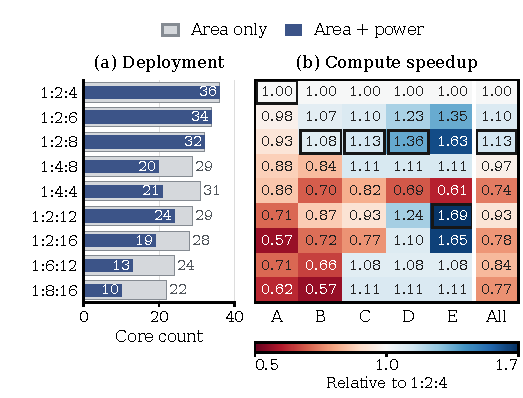
\includegraphics[width=\columnwidth]{v41_case_panels_overlay.pdf}
\caption{固定预算下的部署规模与负载收益（$\alpha=0.327$，$\beta=1$）。(a) 灰色为仅面积约束的核数，蓝色为面积、功耗联合约束的核数。(b) 五阶段迁移的理想 GEMM 计算加速比；A--E 各等权汇总 11 个上下文，All 汇总 55 个组合，黑框标记各列最优值。}
\label{fig:fixed_budget_compact}
\end{figure}

图~\ref{fig:fixed_budget_compact}(b) 表明，在本案例的面积与严格功耗约束下，大幅增加低精度算力的配比未取得综合优势；适度 FP4 增配的 $1:2:8$ 取得最佳综合收益，相对 $1:2:4$ 的理想 GEMM 计算加速比为 $1.13\times$。在相同预算下，$1:2:8$ 保留较高部署密度与高精度吞吐，兼顾低精度增益和剩余混合精度工作量。
